\documentclass[a4paper,zihao=5,UTF8]{ctexart}
\usepackage[top=2.3cm,bottom=2cm,left=1.7cm,right=1.7cm]{geometry} 
\usepackage{amsmath, amssymb}
\usepackage{color}
\usepackage{hyperref} 
\usepackage{pythonhighlight}
\usepackage{listings}
\usepackage{mathrsfs} 
\usepackage{booktabs}
\usepackage{amsthm}
\usepackage{longtable} 
\usepackage{graphicx}
\usepackage{subfigure}
\usepackage{caption}
\usepackage{fontspec}
\usepackage{titlesec}
\usepackage{fancyhdr}
\usepackage{latexsym}
\usepackage{braket}
\usepackage{cite}
\usepackage[version=4]{mhchem}
\usepackage{makecell}
\usepackage{listings}
\usepackage{bm}

\lstset{
 columns=fixed,       
 numbers=left,                                        % 在左侧显示行号
 numberstyle=\tiny\color{gray},                       % 设定行号格式
 frame=none,                                          % 不显示背景边框
 backgroundcolor=\color[RGB]{245,245,244},            % 设定背景颜色
 keywordstyle=\color[RGB]{40,40,255},                 % 设定关键字颜色
 numberstyle=\footnotesize\color{darkgray},           
 commentstyle=\it\color[RGB]{0,96,96},                % 设置代码注释的格式
 stringstyle=\rmfamily\slshape\color[RGB]{128,0,0},   % 设置字符串格式
 showstringspaces=false,                              % 不显示字符串中的空格
 language=c++,                                        % 设置语言
}

\CTEXsetup[format={\Large\bfseries}]{section}
\def\d{\mathrm{d}}
\def\e{\mathrm{e}}
\def\i{\mathrm{i}}
\def\dps{\displaystyle}
\newcommand{\mr}[1]{\mathrm{#1}}
\newcommand{\mb}[1]{\mathbf{#1}}
\newcommand{\dv}[2]{\frac{\d{#1}}{\d{#2}}}
\newcommand{\pdv}[2]{\frac{\partial{#1}}{\partial{#2}}}
\def\degree{$^{\circ}$}
\def\celsius{^{\circ}\mr{C}}
\title{\textbf{Hofstadter蝴蝶}}
\author{王崇斌\;1800011716}
\makeatletter
\makeatother
\begin{document}
	\pagestyle{fancy}
	\pagestyle{fancy}
    \lhead{计算物理A}
	\chead{}
	\rhead{\today}
	\maketitle
    \thispagestyle{fancy}
    \tableofcontents
    \section{题目描述1}
	环形弹簧振子链的运动方程可以写为:
	\begin{equation}
		\left\{
			\begin{aligned}
				m\ddot{x}_{i} &= \kappa(x_{i+1} - x_{i}) + \kappa(x_{i - 1} - x_{i})\\
				x_{k} &= x_{k + n}
			\end{aligned}
		\right.
	\end{equation}
    通过引入向量$\bm{x} = (x_1, \cdots, x_n)^{\mr{t}}$, 可以将上述耦合的二阶微分方程组写为矩阵的形式:
	\begin{equation}
		\ddot{\bm{x}} + \omega_0 \mb{K}\bm{x} = \mb{0}
	\end{equation}
	其中对称矩阵$\mb{K}$:
	\begin{equation}
		\mb{K} = 
		\begin{pmatrix}
			2 & -1 &  & & -1\\
			-1 & 2 & -1 & & \\
			& -1 & \ddots & \ddots & \\
			 & & \ddots & &-1\\
			 -1 & & & -1 & 2\\
		\end{pmatrix}
	\end{equation}
	求解上述方程的方式是利用相似变换将线性方程组变为对角的形式, 如果$\mb{K} = \mb{Q}^{\mr{t}}\mb{D}\mb{Q}$, 
	上述微分方程可以写为:
	\begin{equation}
		\left[\frac{\d^2}{\d t^2} + \omega_0^2\mb{D}\right]\mb{Q}\bm{x} = \mb{0}
	\end{equation}
	定义新的变量$\bm{y} = \mb{Q}\bm{x}$, 可以将原来的耦合微分方程组化为独立的微分方程, 
	这样就将一个常系数线性微分方程组求解问题转化为了矩阵对角化的问题, 可以用本章学习的知识解决.
	\subsection{数值求解本征值并与解析解比较}
	\paragraph{问题:}数值求解$n=2, 16, 128, 1024$的矩阵本征值, 并与解析结果比较:
	\begin{equation}
		\lambda_k = 2\left(1 - \cos\frac{2\pi k}{n}\right)
	\end{equation}
	\paragraph{解:}本题中的代码参见1\_eigenvalue.cpp文件, 其中调用了自己编写的数值线性代数程序
	My\_Matrix.cpp 和 My\_Matrix.h, 输出会被存储在二进制文件.dat中. 求对称矩阵特征值的算法: 首先使用Householder变换将对称矩阵
	通过正交相似变换变为对称三对角矩阵, 再对已经三对角化的矩阵使用Wilkinson位移的QR迭代, 其中QR
	分解使用Givens变换实现(这一步参考了数值线性代数教材上的算法, 将QR分解隐含在了迭代中).
	\par 
	经过数值实验发现, 位移QR迭代收敛极快, 基本上可以在$O(n)$的迭代步数内收敛到机械精度(对n=1000实践发现
	大概900-1000次迭代就收敛), 而三对角矩阵QR迭代一步的复杂度是$O(n)$, 那么基本上可以在$O(n^2)$的
	复杂度下实现QR迭代求解三对角矩阵特征值问题. 主要消耗时间的是Householder变换, 这一步消耗为$O(n^3)$, 
	如果对于大型矩阵可以减少这一步的消耗, 那么通过带位移的QR迭代求解矩阵本征值将会是非常迅速的. 本次作业
	中的矩阵非常接近三对角矩阵, 但是我还是没有设计处针对这种矩阵的特殊算法, 只能先用Householder变换
	凑活一下了. 
	\par 
	首先$n = 2$时矩阵有形式:
	\begin{equation}
		\mb{K} = 
		\begin{pmatrix}
			2 & -1\\
			-1 & 2
		\end{pmatrix}
	\end{equation}
	容易直接计算这个矩阵的本征值是$3, 1$, 并不符合题目中给出的公式, 这与两个原子无法形成环形
	振子链是一致的,题目中的公式应该是对于$n>=3$的情况成立. 对于$n>2$的情况, 考虑采用将本征值排序并
	绘图的方式比较我的算法与解析值的差异(参见图\ref{1 eig diff plot}), 此外计算数值本征值序列和解析本征值序列差的一范数(参见
	表\ref{1 eig diff table}), 
	用于衡量数值和解析的差异.
	\begin{table}[htbp]
		\centering
		\caption{数值本征值向量与解析本征值向量差的一范数}
		\begin{tabular}[htbp]{ccccc}
			\toprule
			$n$ & 3& 16& 128& 1024 \\
			\midrule
			diff & $4.44\times10^{-16}$& $1.71\times10^{-14}$& $3.29\times10^{-13}$& $3.83\times10^{-12}$ \\
			\bottomrule
		\end{tabular}
		\label{1 eig diff table}
	\end{table}
	\begin{table}[htbp]
		\centering
		\begin{tabular}[htbp]{cc}
			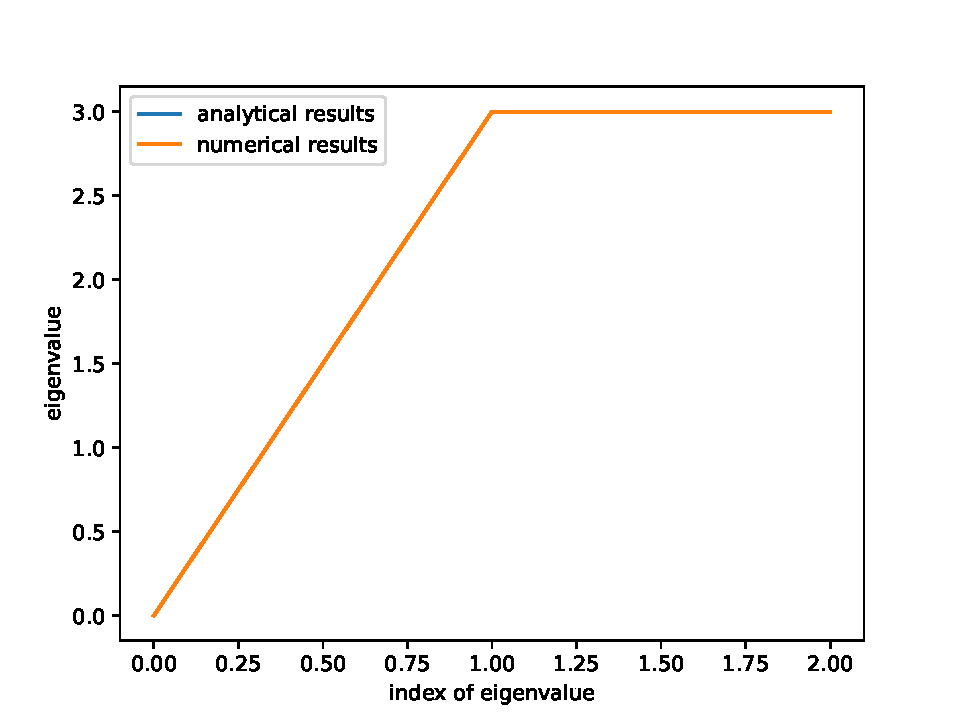
\includegraphics[scale=0.5]{1_compare_n=3.pdf} & 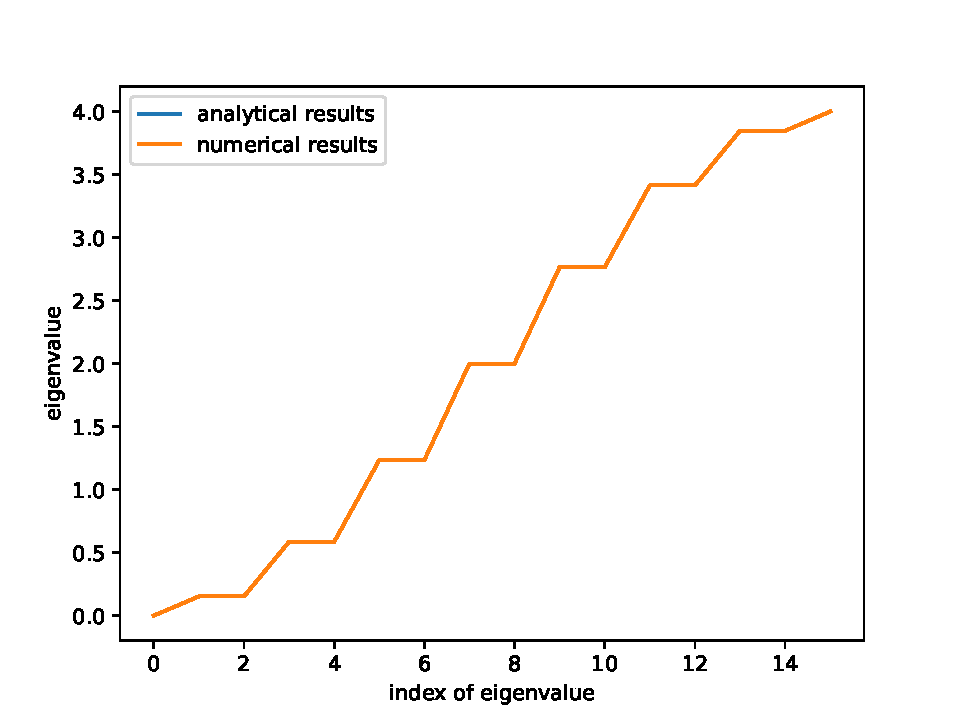
\includegraphics[scale=0.5]{1_compare_n=16.pdf}\\
			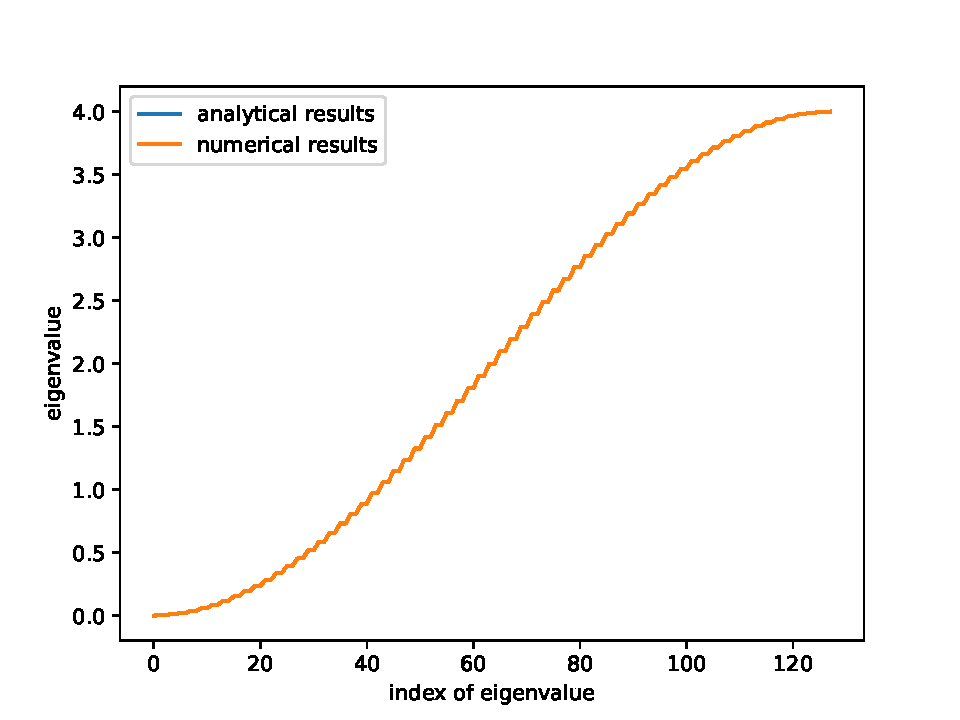
\includegraphics[scale=0.5]{1_compare_n=128.pdf} & 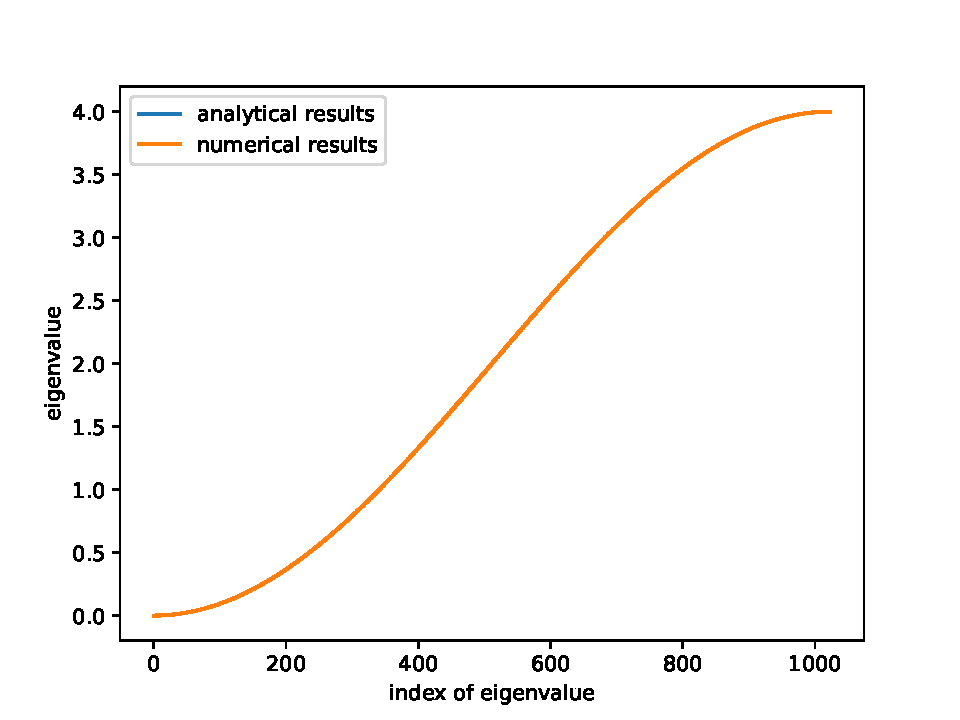
\includegraphics[scale=0.5]{1_compare_n=1024.pdf}\\
		\end{tabular}
		\caption{数值本征值和解析本征值的比较}
		\label{1 eig diff plot}
	\end{table}
	
	\section{题目描述2}
	由于矩阵本身的特殊性, 可以方便地写出本征值满足的方程:
	\begin{equation}
		-x_{j-1} + 2x_{j} - x_{j+1} = \lambda x_{j}
	\end{equation}
	上式可以写成传输矩阵的形式:
	\begin{equation}
		\begin{pmatrix}
			x_{j+1}\\
			x_{j}
		\end{pmatrix} = 
		\begin{pmatrix}
			2-\lambda & -1\\
			1 & 0\\
		\end{pmatrix}
		\begin{pmatrix}
			x_j\\
			x_{j-1}
		\end{pmatrix}
	\end{equation}
	那么:
	\begin{equation}
		\begin{pmatrix}
			x_{j+n}\\
			x_{j+n-1}
		\end{pmatrix}=
		\begin{pmatrix}
			2-\lambda & -1\\
			1 & 0\\
		\end{pmatrix}^{n}
		\begin{pmatrix}
			x_j\\
			x_{j-1}
		\end{pmatrix}
	\end{equation}
	只要将上述矩阵的特征值求出, 同时利用周期边界条件, 就可以方便地求出$\lambda$的值, 从而得到
	原矩阵$\mb{K}$的本征值.
	\par 
	如果给每个振子额外加上一根劲度系数周期变化的弹簧, 系统的运动方程变为:
	\begin{equation}
		m\ddot{x}_{j} = \kappa(x_{j + 1} - x_j) + \kappa(x_{j - 1} - x_{j}) - 
		[g_0 - g_1\cos(2\pi j\alpha)]x_j
	\end{equation}
	那么容易验证, 新的矩阵相当于在原矩阵对角元上加上了一项. 此时系统的本征值方程可以写为
	(不妨假设$\kappa=1, m=1$):
	\begin{equation}
		x_{j+1} = \left[2 - \lambda + g_0 + g_1\cos(2\pi j\alpha)\right]x_j - x_{j-1}
	\end{equation}

	\subsection{数值求解矩阵的本征值并观察本征值的分布}
	\paragraph{问题:}取$\gamma = g_1/\kappa = 2,\,\alpha=0.5,\,n=720$, 
	直接对角化$\mb{K}$, 验证$c:=2-\lambda + g_0/\kappa$分布在两个分立的区间中.
	\paragraph{解:}
	为了方便起见将$g_0$设为0. 在数值测试的时候发现当矩阵变大时自己的QR迭代收敛性很差, 
	可以观察到从某个矩阵阶数之后迭代就不再收敛(但是在这个临界值之前迭代会以$O(n)$的速度收敛), 
	在反复确认了自己的代码没有问题之后(通过比较收敛的结果的正确性和检查代码本身), 我将
	目光投向了数值精度问题, 发现在更改了一些"x==0"的判断条件, 将其改为$\mr{abs}(x) < \delta$之后, 
	改变$\delta$的值对结果的收敛性有比较大的影响, 因此我抱着试一试的态度将原来代码中的浮点数类型
	从double改为了long double, 结果收敛性得到了明显地改善, 同时也没有增加太多运算时间. 
	\par 
	将求解出的本征值排序, 将$C = 2 - \lambda$绘制在图中, 参见图\ref{2 eigenvalue}, 可以明显看出取值劈裂
	在了两个区间中.
	\begin{figure}[htbp]
		\centering
		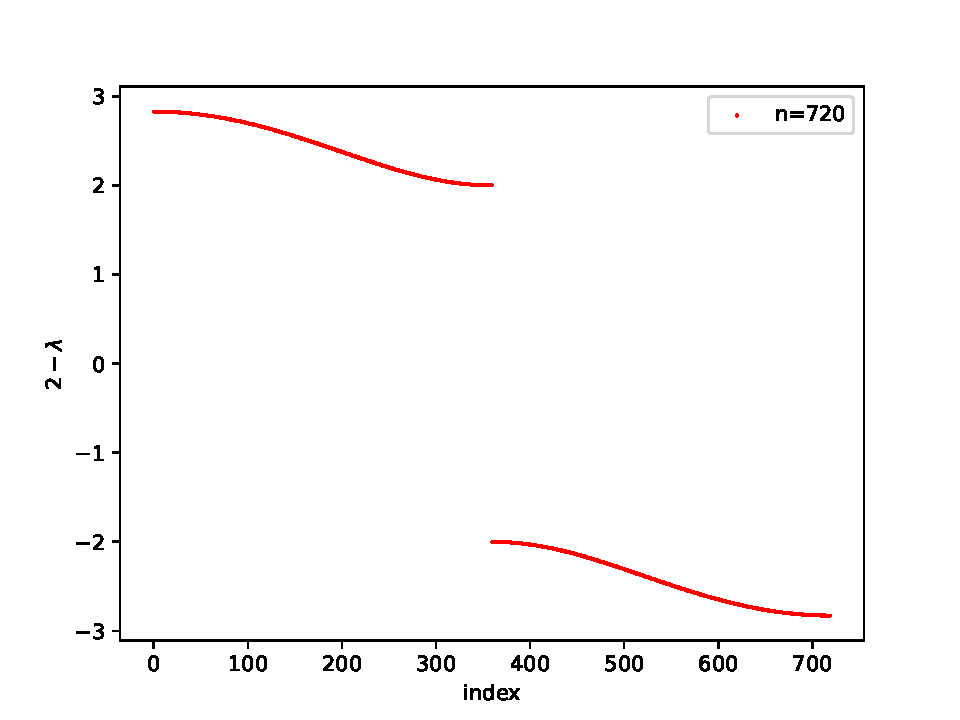
\includegraphics[scale=0.6]{2_eigenvalue.pdf}
		\caption{$n=720$时$c-\lambda$的分布}
		\label{2 eigenvalue}
	\end{figure}

	\subsection{矩阵本征值的解析解}
	考虑使用第二题中的参数$\alpha = 0.5$, 首先对于普遍的情况给出传输矩阵的表达式, 定义
	$f(j) = c + \gamma\cos(2\pi j \alpha)$:
	\begin{equation}
		\left\{
			\begin{aligned}
				x_{j + 2} &= f(j + 1)\left[f(j)x_j - x_{j - 1}\right] - x_j\\
				x_{j +1} &= f(j)x_j- x_{j - 1}\\
				x_j &= f(j - 1)x_{j - 1} - x_{j-2}
			\end{aligned}
		\right.
	\end{equation} 
	上述表达式容易写为矩阵方程:
	\begin{equation}
		\begin{pmatrix}
			x_{j+2}\\
			x_{j + 1}\\
			x_{j}
		\end{pmatrix}
		=
		\begin{pmatrix}
			f(j+1)f(j) - 1 & -f(j+1) &0 \\
			f(j) & -1 & 0\\
			0 & f(j-1) & -1
		\end{pmatrix}
		\begin{pmatrix}
			x_{j}\\
			x_{j-1}\\
			x_{j-2}
		\end{pmatrix}
	\end{equation}
	将参数$\alpha=0.5$带入之后矩阵方程可以表达为:
	\begin{equation}
		\begin{pmatrix}
			x_{j+2}\\
			x_{j + 1}\\
			x_{j}
		\end{pmatrix}
		=
		\begin{pmatrix}
			c^2 - \gamma^2 - 1 & -(c + \gamma(-1)^j) &0 \\
			c - \gamma(-1)^j & -1 & 0\\
			0 & c + \gamma(-1)^j & -1
		\end{pmatrix}
		\begin{pmatrix}
			x_{j}\\
			x_{j-1}\\
			x_{j-2}
		\end{pmatrix}
	\end{equation}
	由循环边界条件$x_j = x_{j+n}$可知:
	\begin{equation}
		\begin{pmatrix}
			c^2 - \gamma^2 - 1 & -(c + \gamma(-1)^j) &0 \\
			c - \gamma(-1)^j & -1 & 0\\
			0 & c + \gamma(-1)^j & -1
		\end{pmatrix}^{n/2} = \mb{E}_3
	\end{equation}
	上述矩阵的特征多项式为:
	\begin{equation}
		\begin{aligned}
			p(\mu) &= (c^2 - \gamma^2 - 1 - \mu)(\mu + 1)^2 - (c^2 - \gamma^2)(\mu + 1)\\
			& = \left[\mu(c^2 - \gamma^2) - (\mu + 1)^2\right](\mu + 1)
		\end{aligned}
	\end{equation}
	由于循环边界条件, 上述矩阵的特征多项式零点满足$\mu^{n/2} = 1$, 那么$\mu = \exp(\pm4\pi\i k/n)$
	其中$k$是一个待定的整数. 对$\mu$的约束等价于对$c$的约束, 容易看出, 特征多项式的零点满足:
	\begin{equation}
		\left\{
			\begin{aligned}
				&\mu = -1\\
				&c^2 - \gamma^2 = \frac{(1 + \mu)^2}{\mu}
			\end{aligned}
		\right.
	\end{equation}
	从而可以计算出$c = \pm\sqrt{\gamma^2 + 4\cos(2\pi k / n)}$, 考虑到特征值的个数, k的取值范围应该是$0, n/2$
	之间的所有整数, 将解析特征值与数值特征值画在同一张图上进行比较(图\ref{3 compare}), 特征值之间已经经过了排序.
	\begin{figure}[htbp]
		\centering
		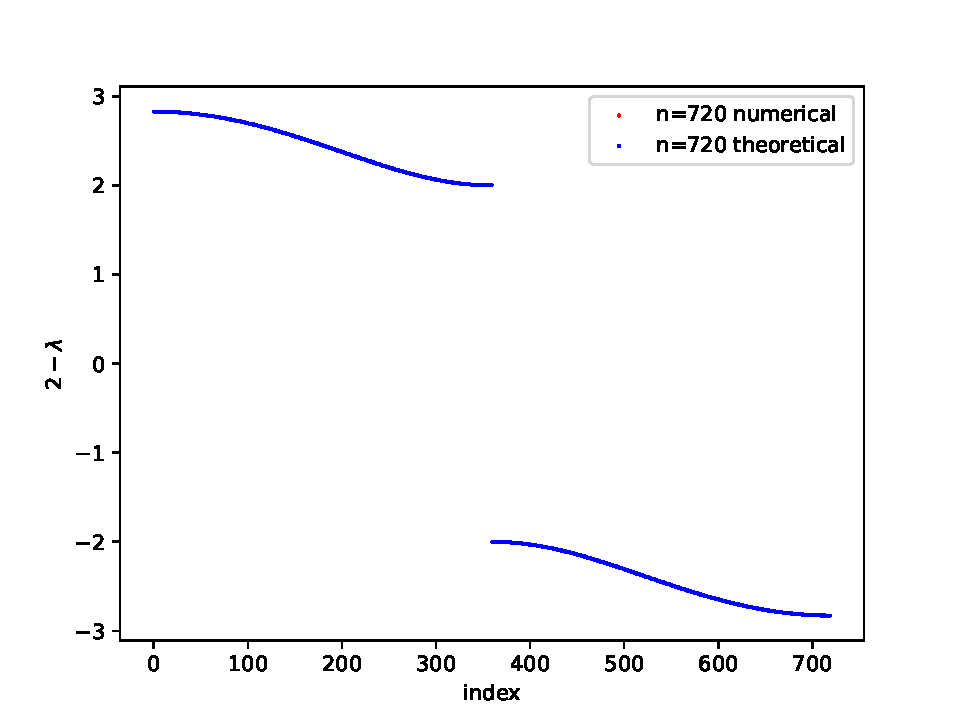
\includegraphics[scale=0.6]{3_compare.pdf}
		\caption{数值本征值与解析本征值之间的比较}
		\label{3 compare}
	\end{figure}
	\subsection{参数$\alpha$取值对于本征值行为的影响}
	\paragraph{$\alpha = 1 / 3$}
	为了方便起见, 这几道题目沿用程序2\_eigenvalue.cpp, 计算时更改其中参数$\alpha$与储存的文件名, 绘图的程序沿用
	2\_plot.py. 取$n=1200$. 图片参见\ref{alpha 1 3}
	\begin{figure}[htbp]
		\centering
		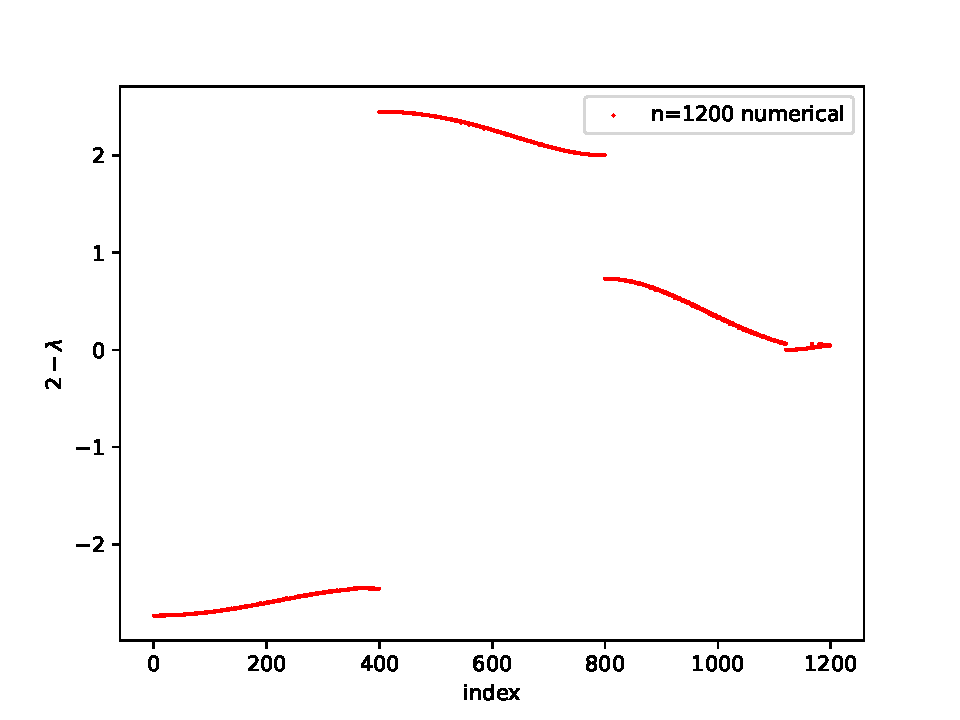
\includegraphics[scale=0.6]{4_alpha_1_3.pdf}
		\caption{$\alpha=1/3$时本征值分裂的情况}
		\label{alpha 1 3}
	\end{figure}
	\paragraph{$\alpha = 1/4$}取$n=1200$, 图片参见\ref{alpha 1 4}
	\begin{figure}[htbp]
		\centering
		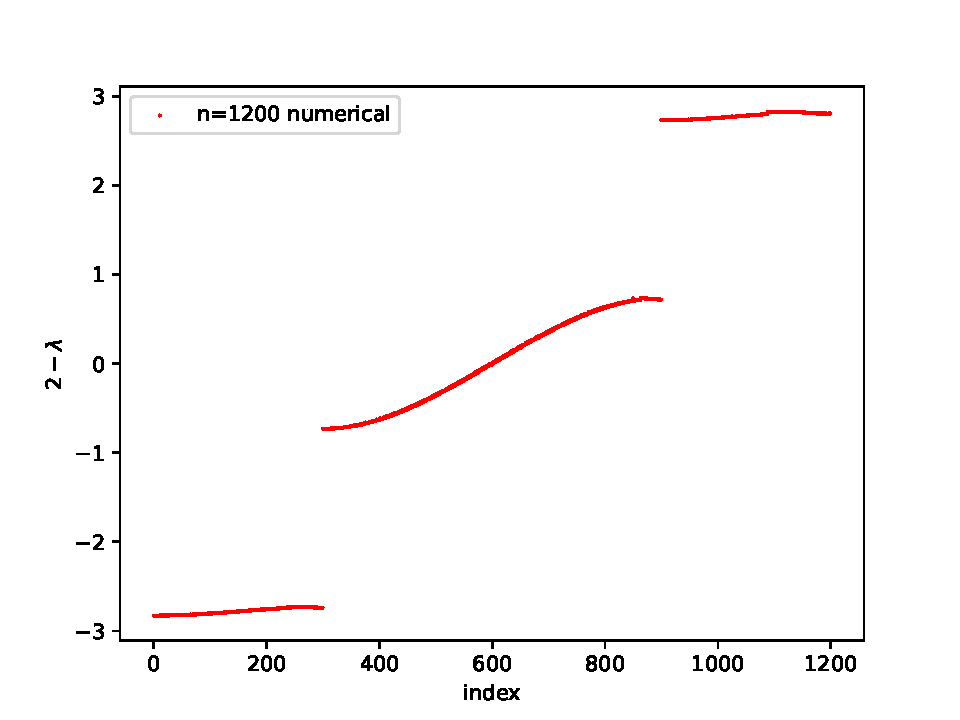
\includegraphics[scale=0.6]{4_alpha_1_4.pdf}
		\caption{$\alpha=1/4$时本征值分裂的情况}
		\label{alpha 1 4}
	\end{figure}
	\paragraph{更多的情况}
	取$\alpha = 2/5, 3/5, 2/7, 3/7, 4/9. 8/9, 9/10, 10/11$观察本征值分裂的情况, $n=1200$, 参见表\ref{diff alpha}
	\begin{table}[htbp]
		\centering
		\begin{tabular}[htbp]{cc}
			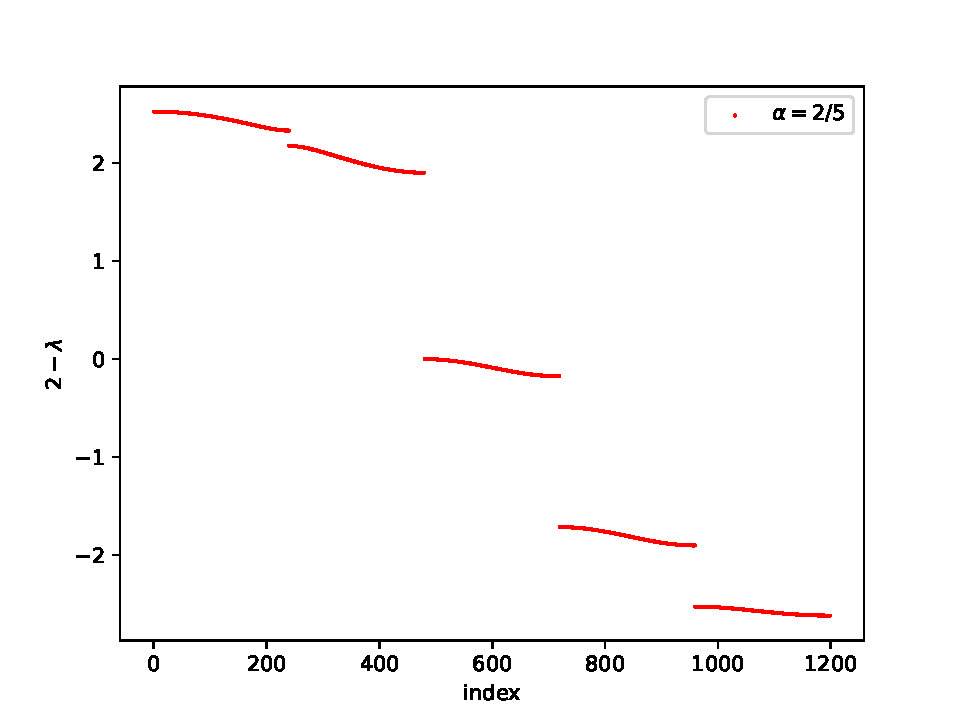
\includegraphics[scale=0.5]{5_alpha_2_5.pdf} & 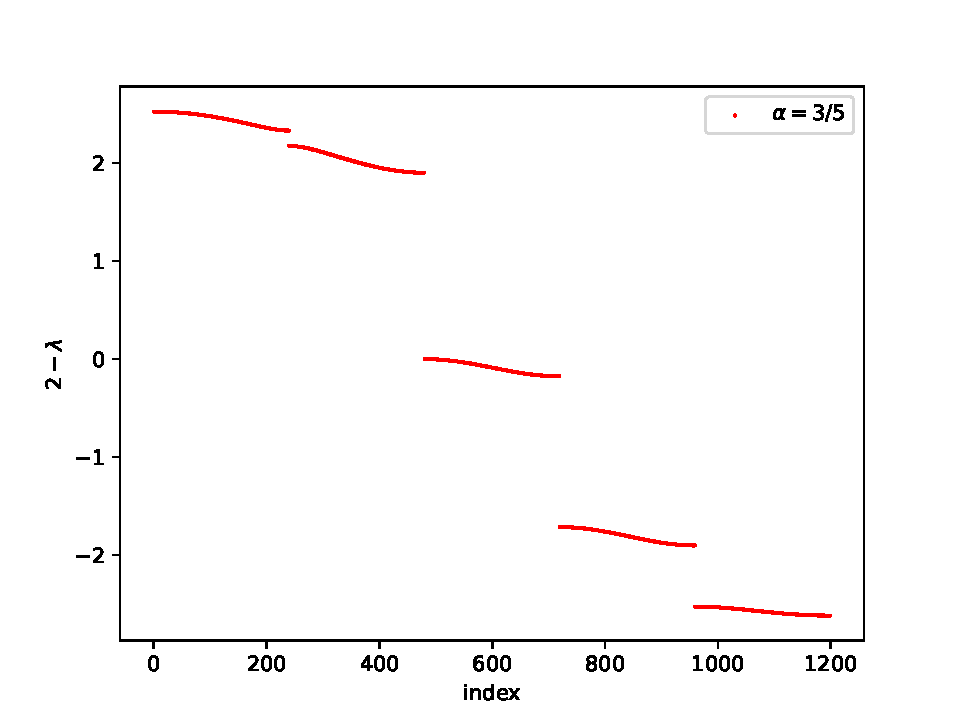
\includegraphics[scale=0.5]{5_alpha_3_5.pdf}\\
			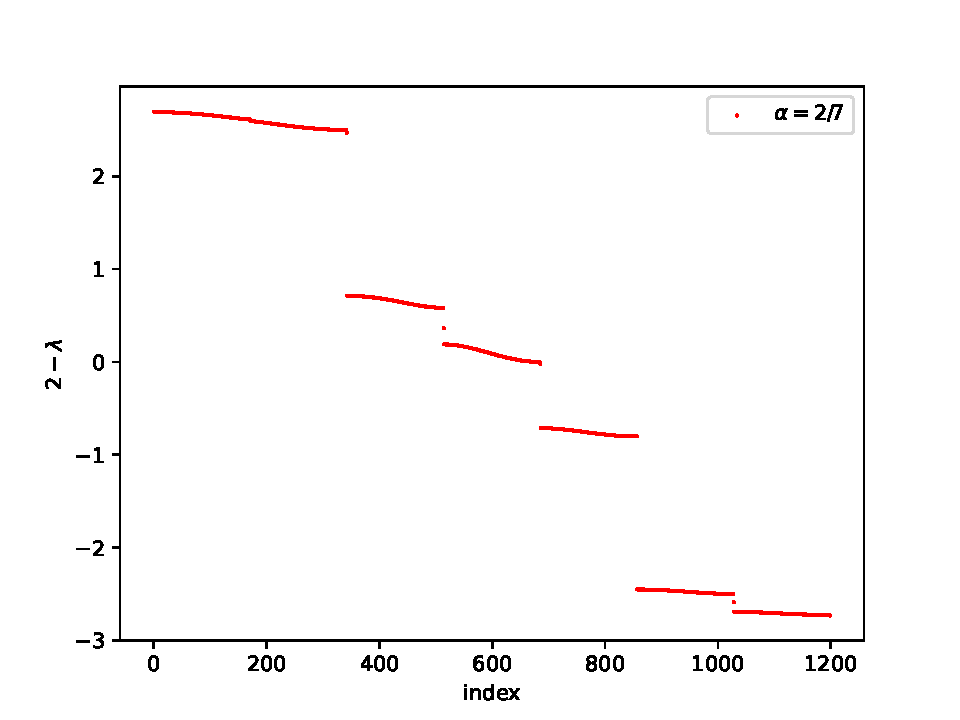
\includegraphics[scale=0.5]{5_alpha_2_7.pdf} & 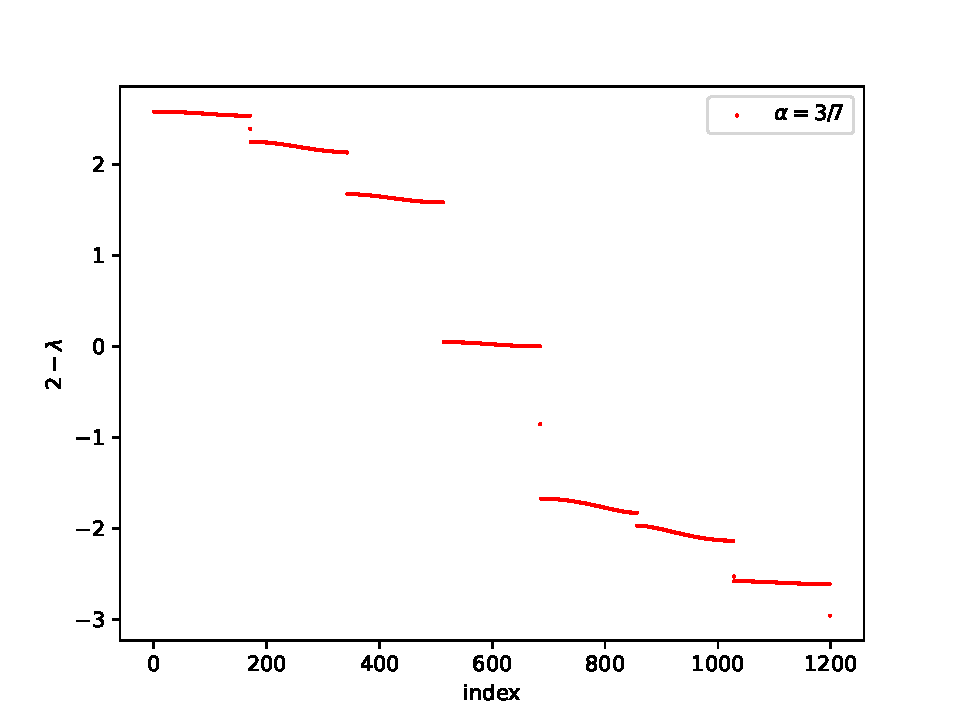
\includegraphics[scale=0.5]{5_alpha_3_7.pdf}\\
			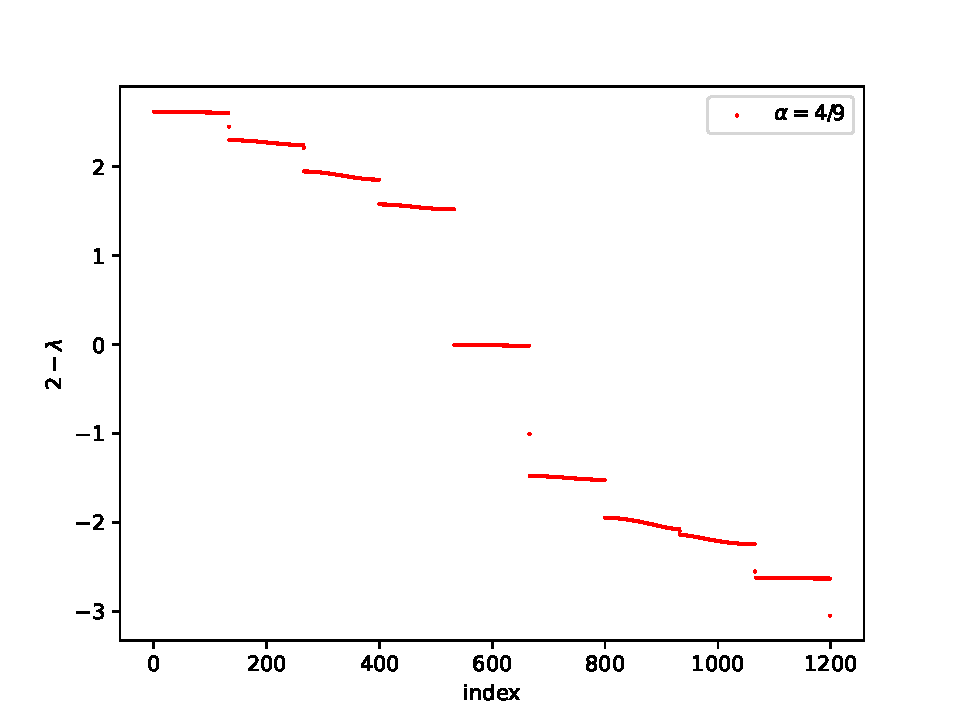
\includegraphics[scale=0.5]{5_alpha_4_9.pdf} & 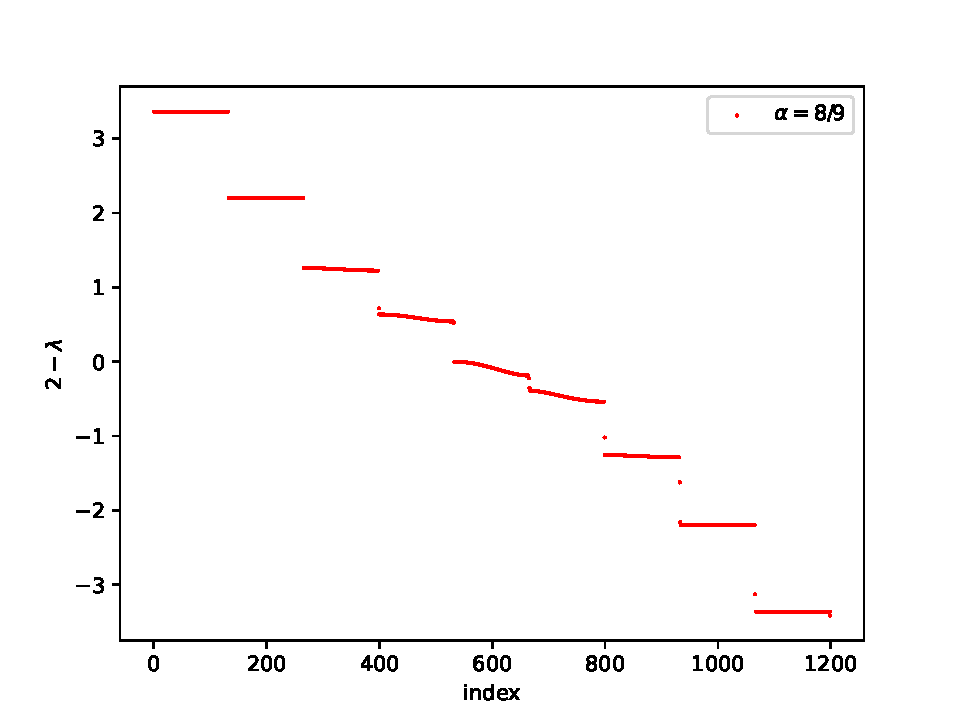
\includegraphics[scale=0.5]{5_alpha_8_9.pdf} \\
			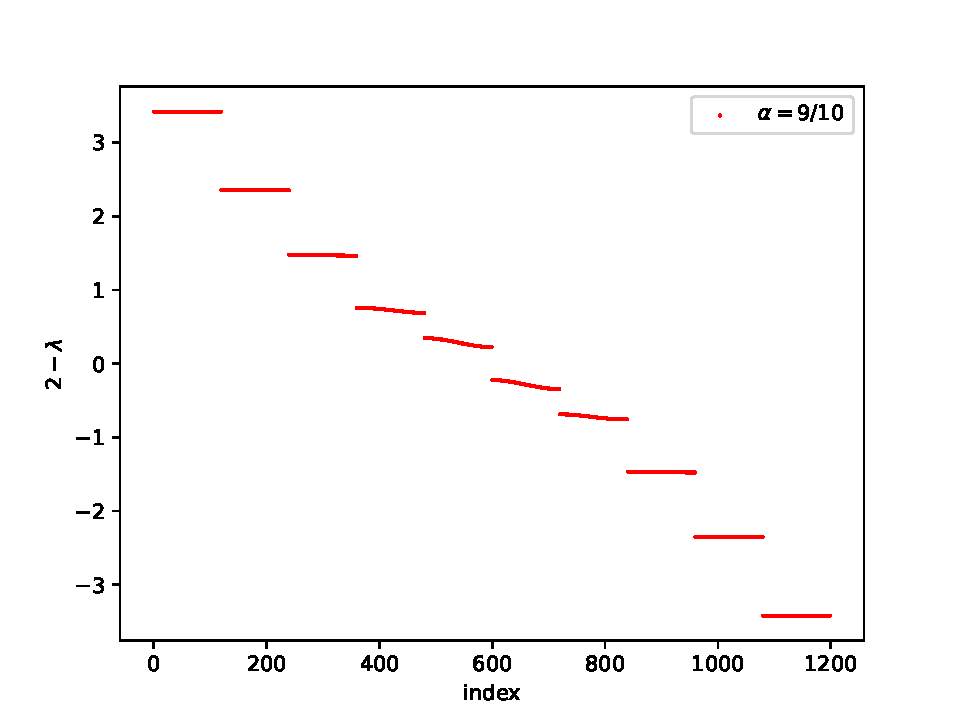
\includegraphics[scale=0.5]{5_alpha_9_10.pdf} & 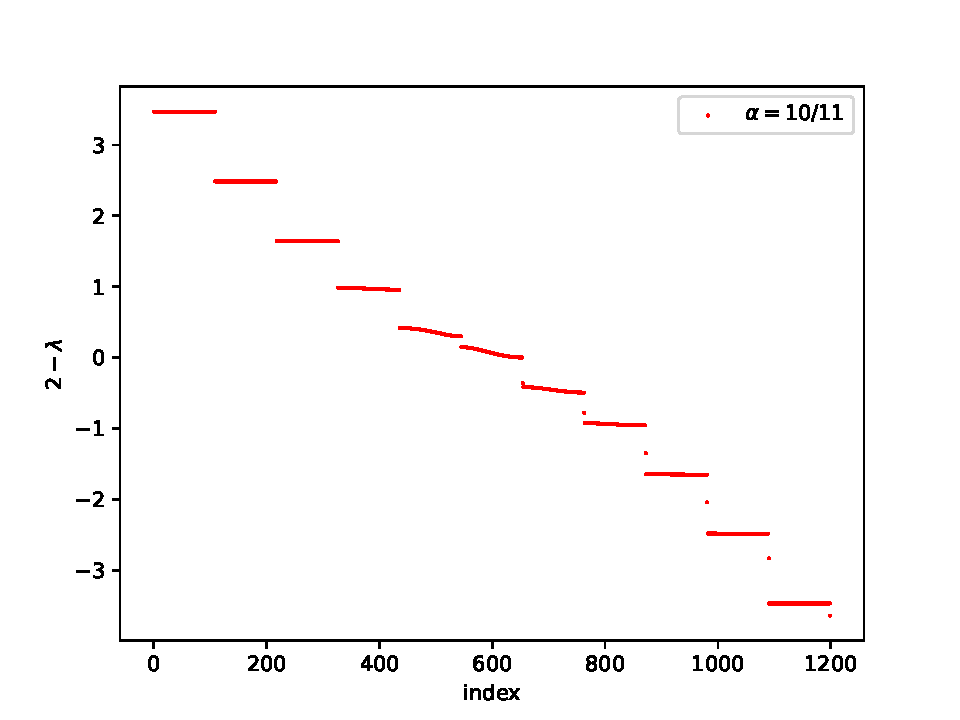
\includegraphics[scale=0.5]{5_alpha_10_11.pdf}\\
		\end{tabular}
		\caption{$\alpha$不同取值时本征值劈裂的情况}
		\label{diff alpha}
	\end{table}
	\subsection{Hofstadter蝴蝶}
	考虑在$[0, 1)$之间等距选取500个点作为$\alpha$的参数, 具体计算程序参见6\_Hofstadter.cpp, 绘图的程序参见6\_plot.py, 
	绘制出的Hofstadter蝴蝶参见\ref{Hofstadter}
	\begin{figure}
		\centering
		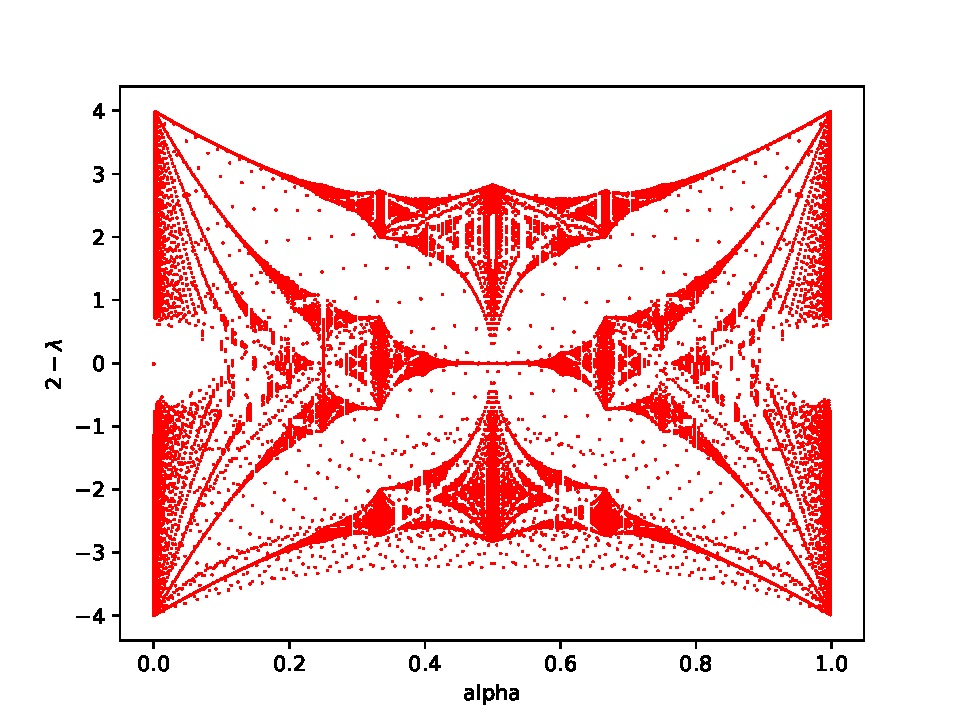
\includegraphics[scale=0.6]{6_Hofstadter_720_500.pdf}
		\caption{Hofstadter蝴蝶}
		\label{Hofstadter}
	\end{figure}
\end{document}